\documentclass{beamer}


\usepackage[utf8]{inputenc}
\usepackage{amsmath}
\usepackage{amsfonts}
\usepackage{amssymb}
\usepackage{graphicx}
\usepackage{ragged2e}  % `\justifying` text
\usepackage{booktabs}  % Tables
\usepackage{tabularx}
\usepackage{tikz}      % Diagrams
\usetikzlibrary{calc, shapes, backgrounds}
\usepackage{amsmath}
\usepackage{amssymb}
\usepackage{dsfont}
\usepackage{url}       % `\url
\usepackage{listings}  % Code listings
\usepackage[T1]{fontenc}
\usepackage[percent]{overpic}
\usetikzlibrary{trees}
\usepackage[absolute,overlay]{textpos}
\usepackage{tcolorbox}



\newtcolorbox{terminal}{colback=black!70!white,colframe=black!70!white}

\usepackage{theme/beamerthemehbrs}

\author[MAS]{Hassan Umari}
\title{ROS Nodes, Topics, and Messages}
\subtitle{Foundation Course}
\institute[HBRS]{Hochschule Bonn-Rhein-Sieg}
\date{\today}
\subject{ROS workshop}

% \thirdpartylogo{path/to/your/image}


\begin{document}
{
\begin{frame}
\titlepage
\end{frame}
}


\section{Recap}
\begin{frame}{Recap}
    \framesubtitle{Summary of yesterday's session}
    \begin{itemize}
        \item ROS is a collection of libraries and tools that helps you when you develop software for robots.
              
        \item ROS provides several ways to transfer data between nodes:
        
        \begin{enumerate}
            \item ROS topics and messages (\textbf{publish/subscribe}).
            \item ROS services (\textbf{request/reply}).
            \item ROS actions (\textbf{request/reply}).
            \item Parameter server.
        \end{enumerate}   
    \end{itemize}
\end{frame}


\begin{frame}{Recap}
    \framesubtitle{Summary of yesterday's session}
    \begin{itemize}
        \item We will focus today on ROS topics and messages..
    \end{itemize}
\end{frame}


     \begin{frame}[plain]{}
         \centering
         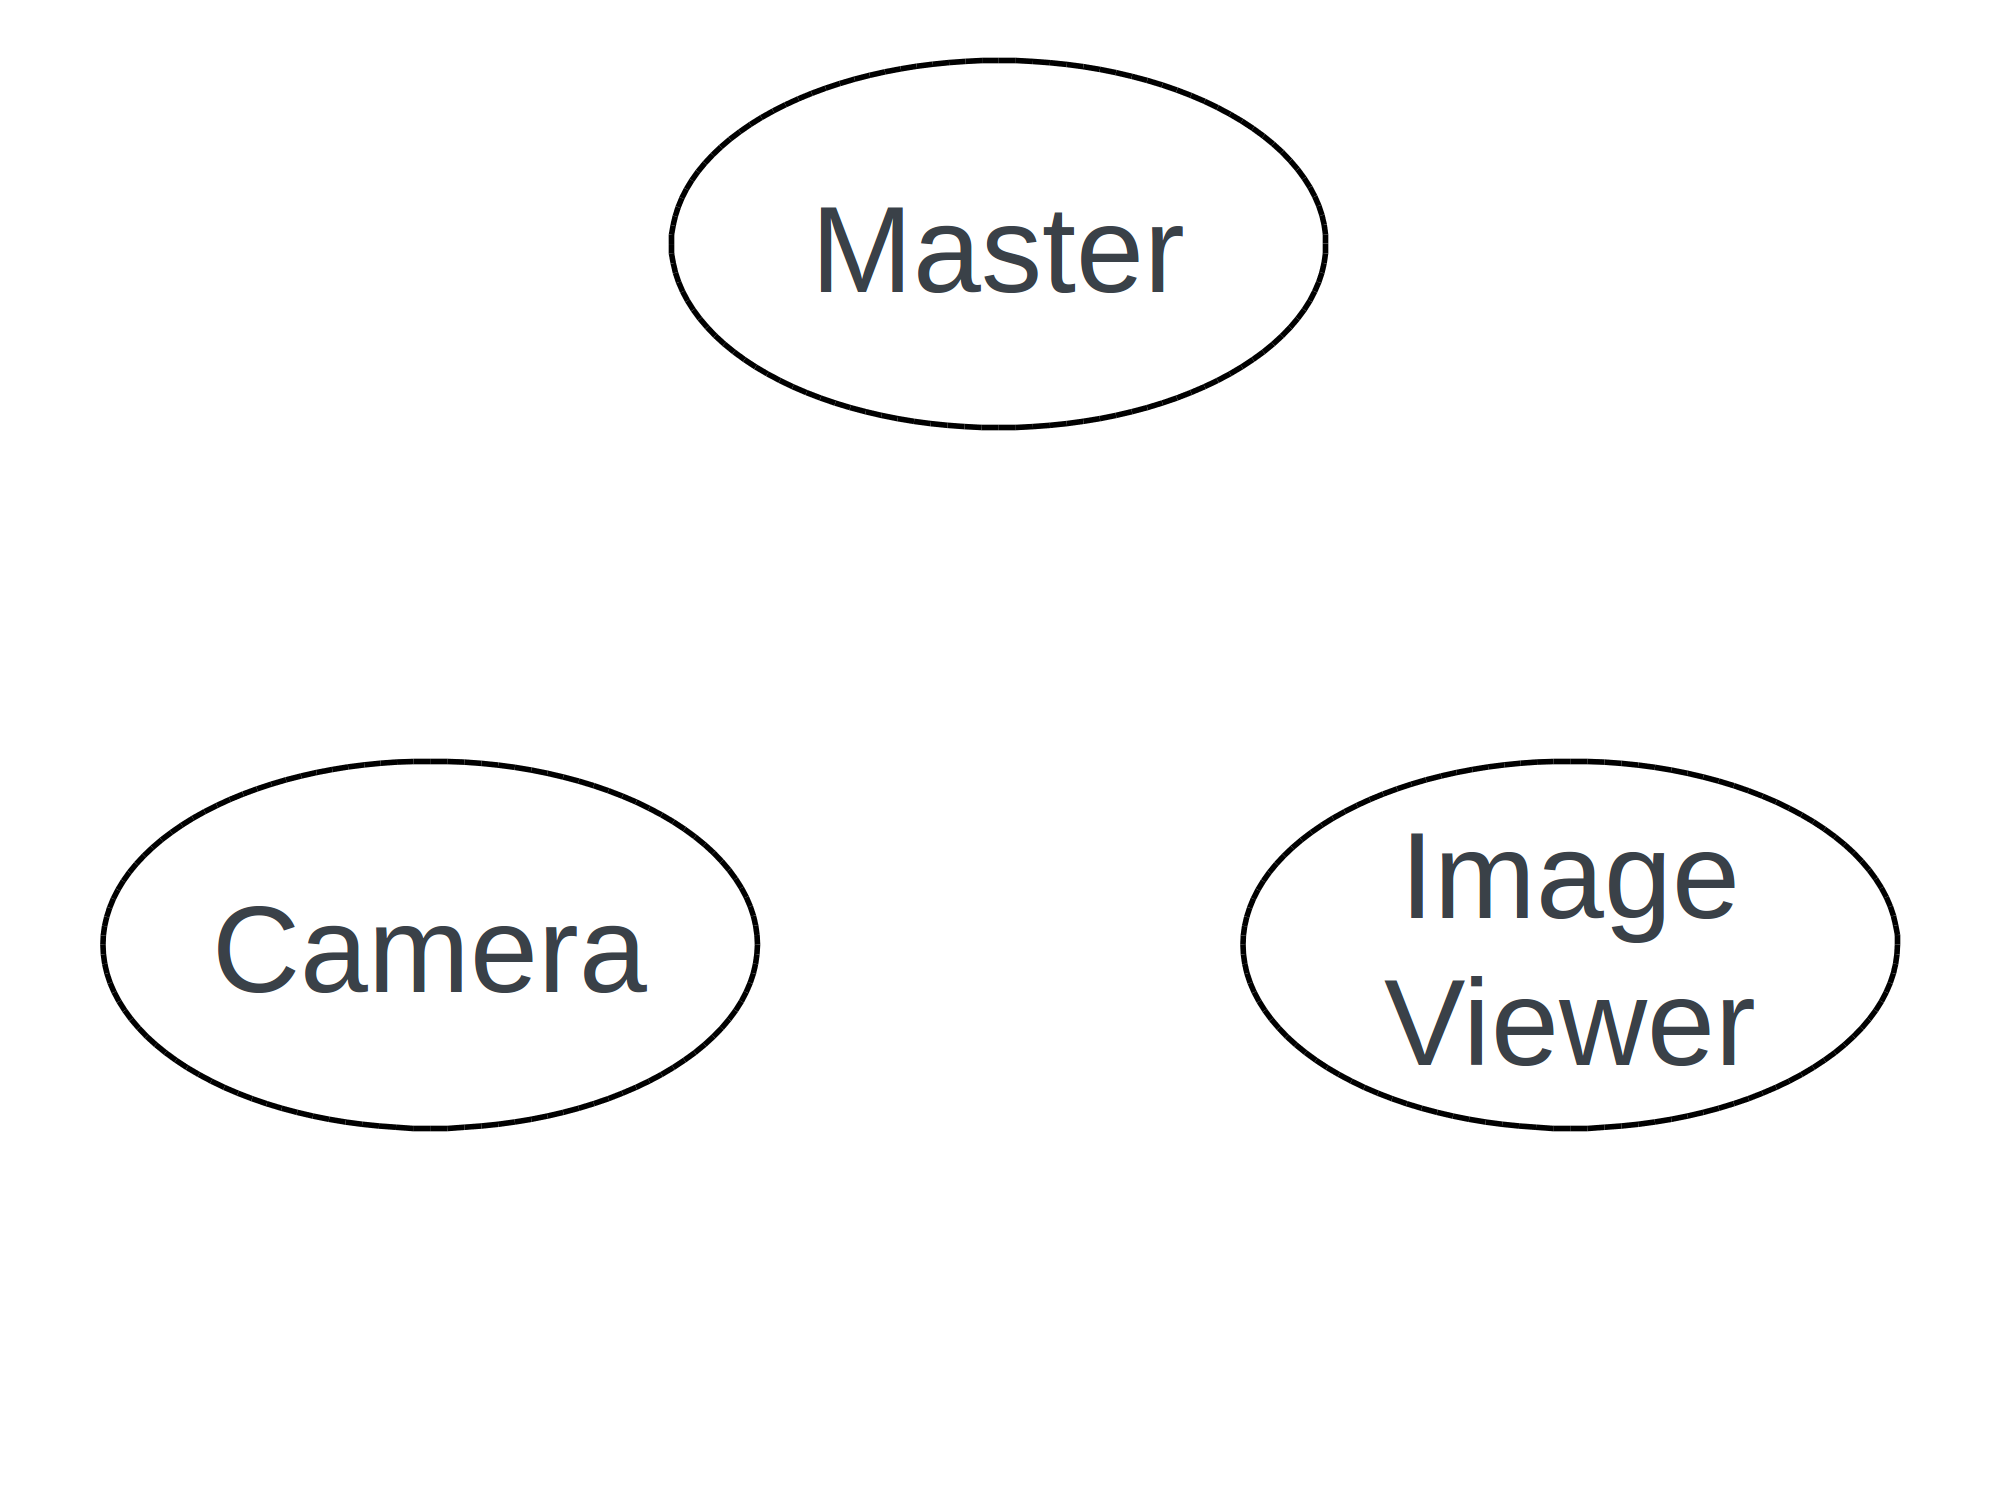
\includegraphics[width =1.0\linewidth]{figures/master1.png}                                                              
        \end{frame} 
        \begin{frame}[plain]{}
            \centering
            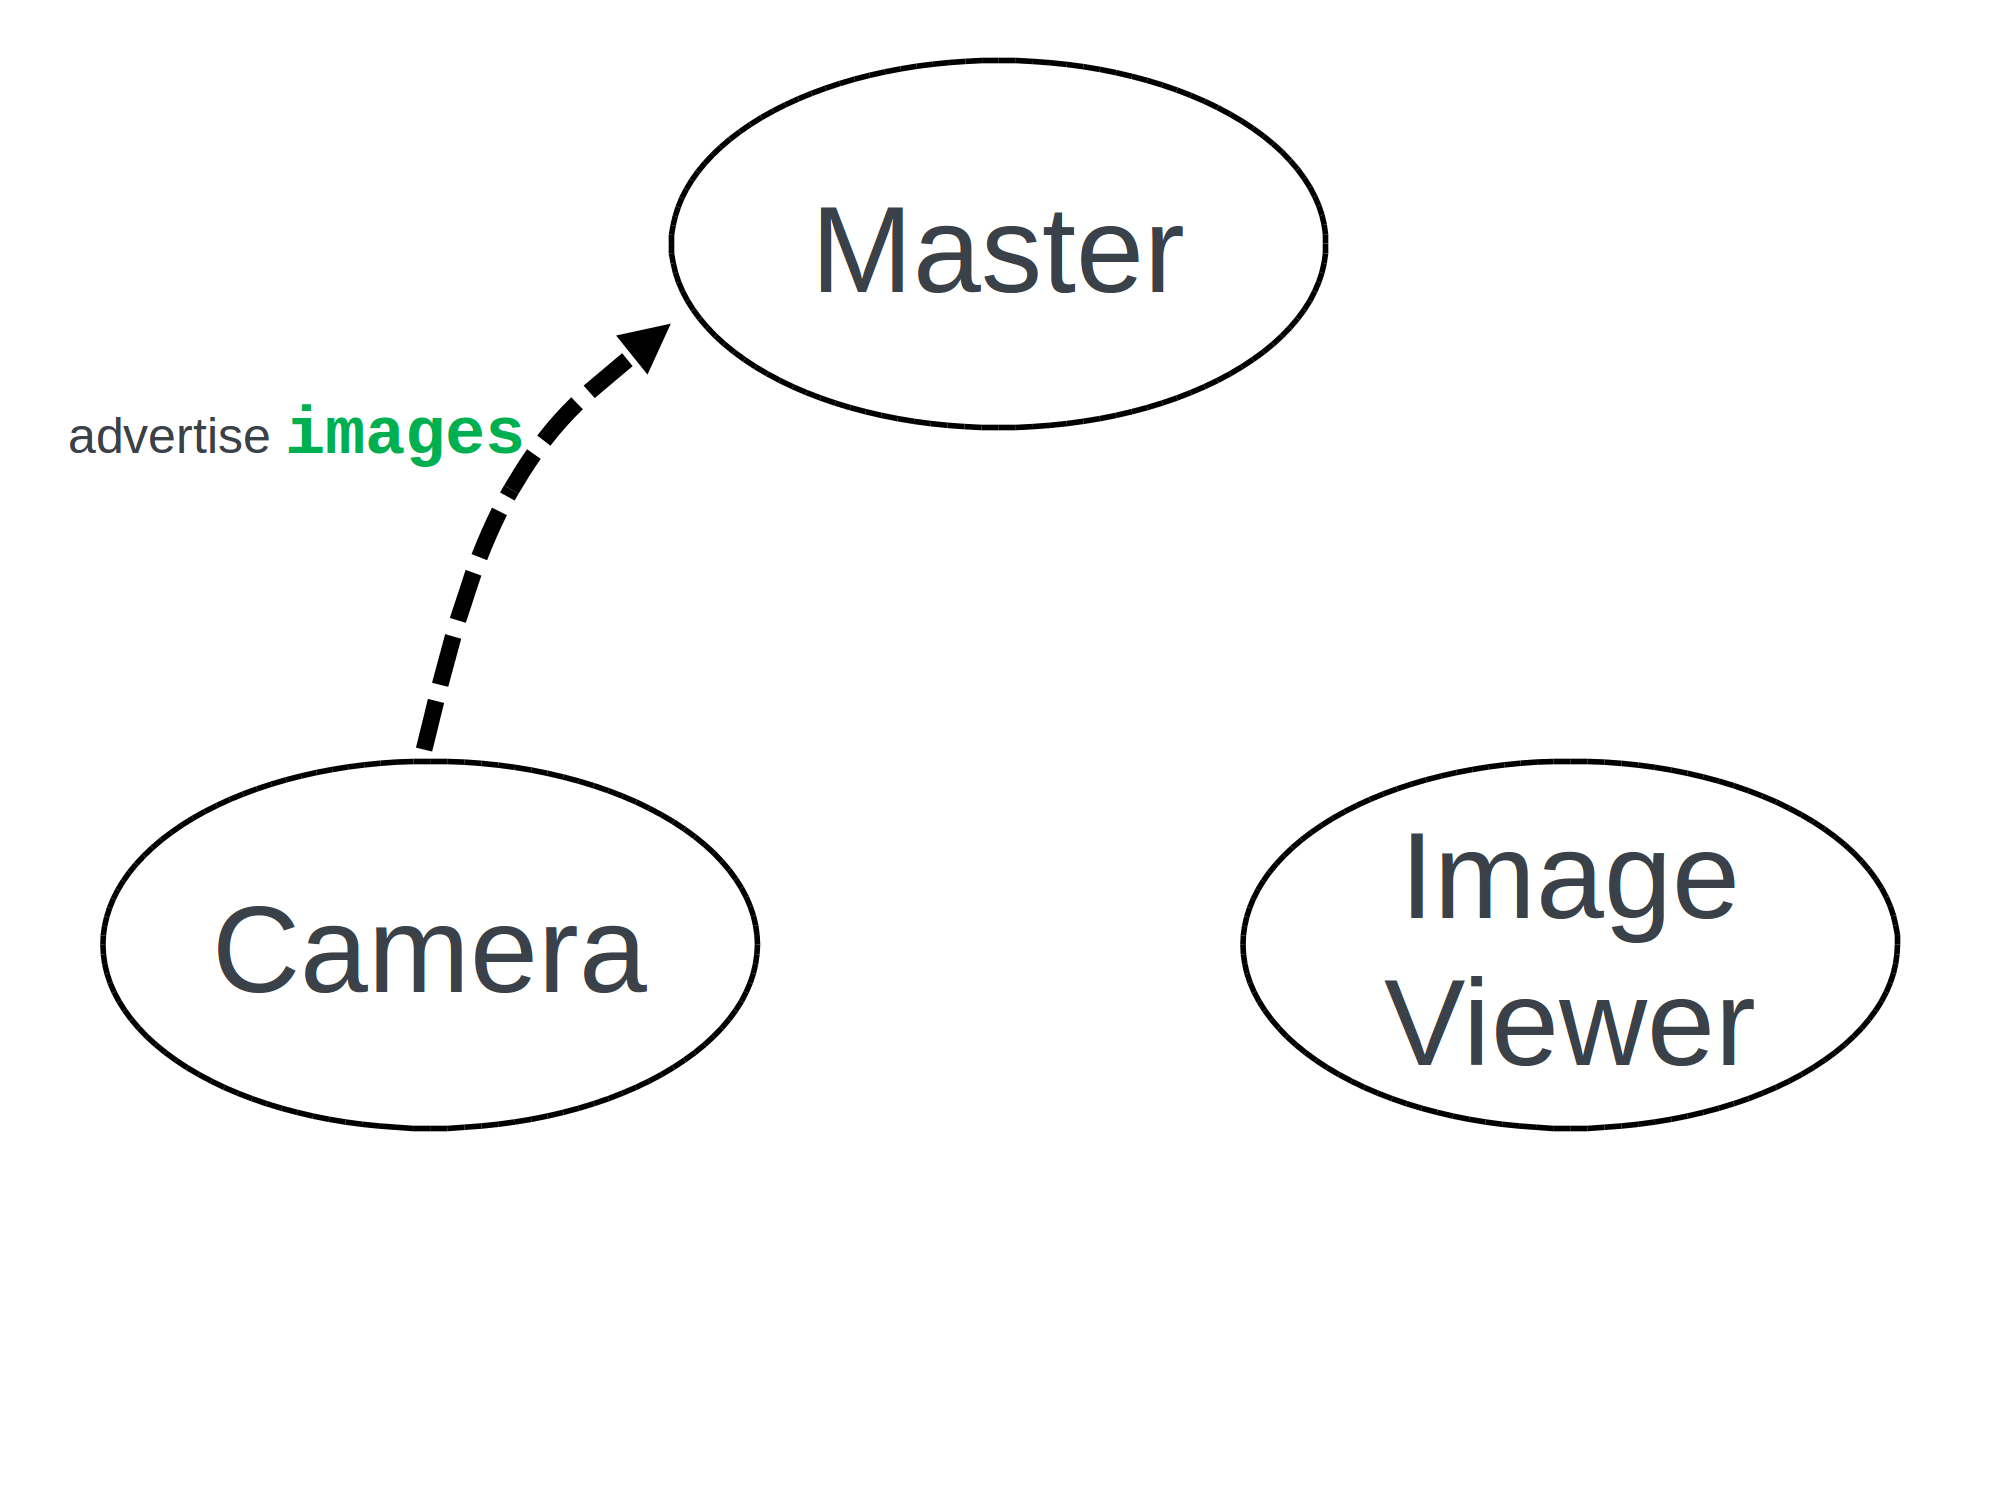
\includegraphics[width =1.0\linewidth]{figures/master2.png}                                                              
        \end{frame} 
        \begin{frame}[plain]{}
            \centering
            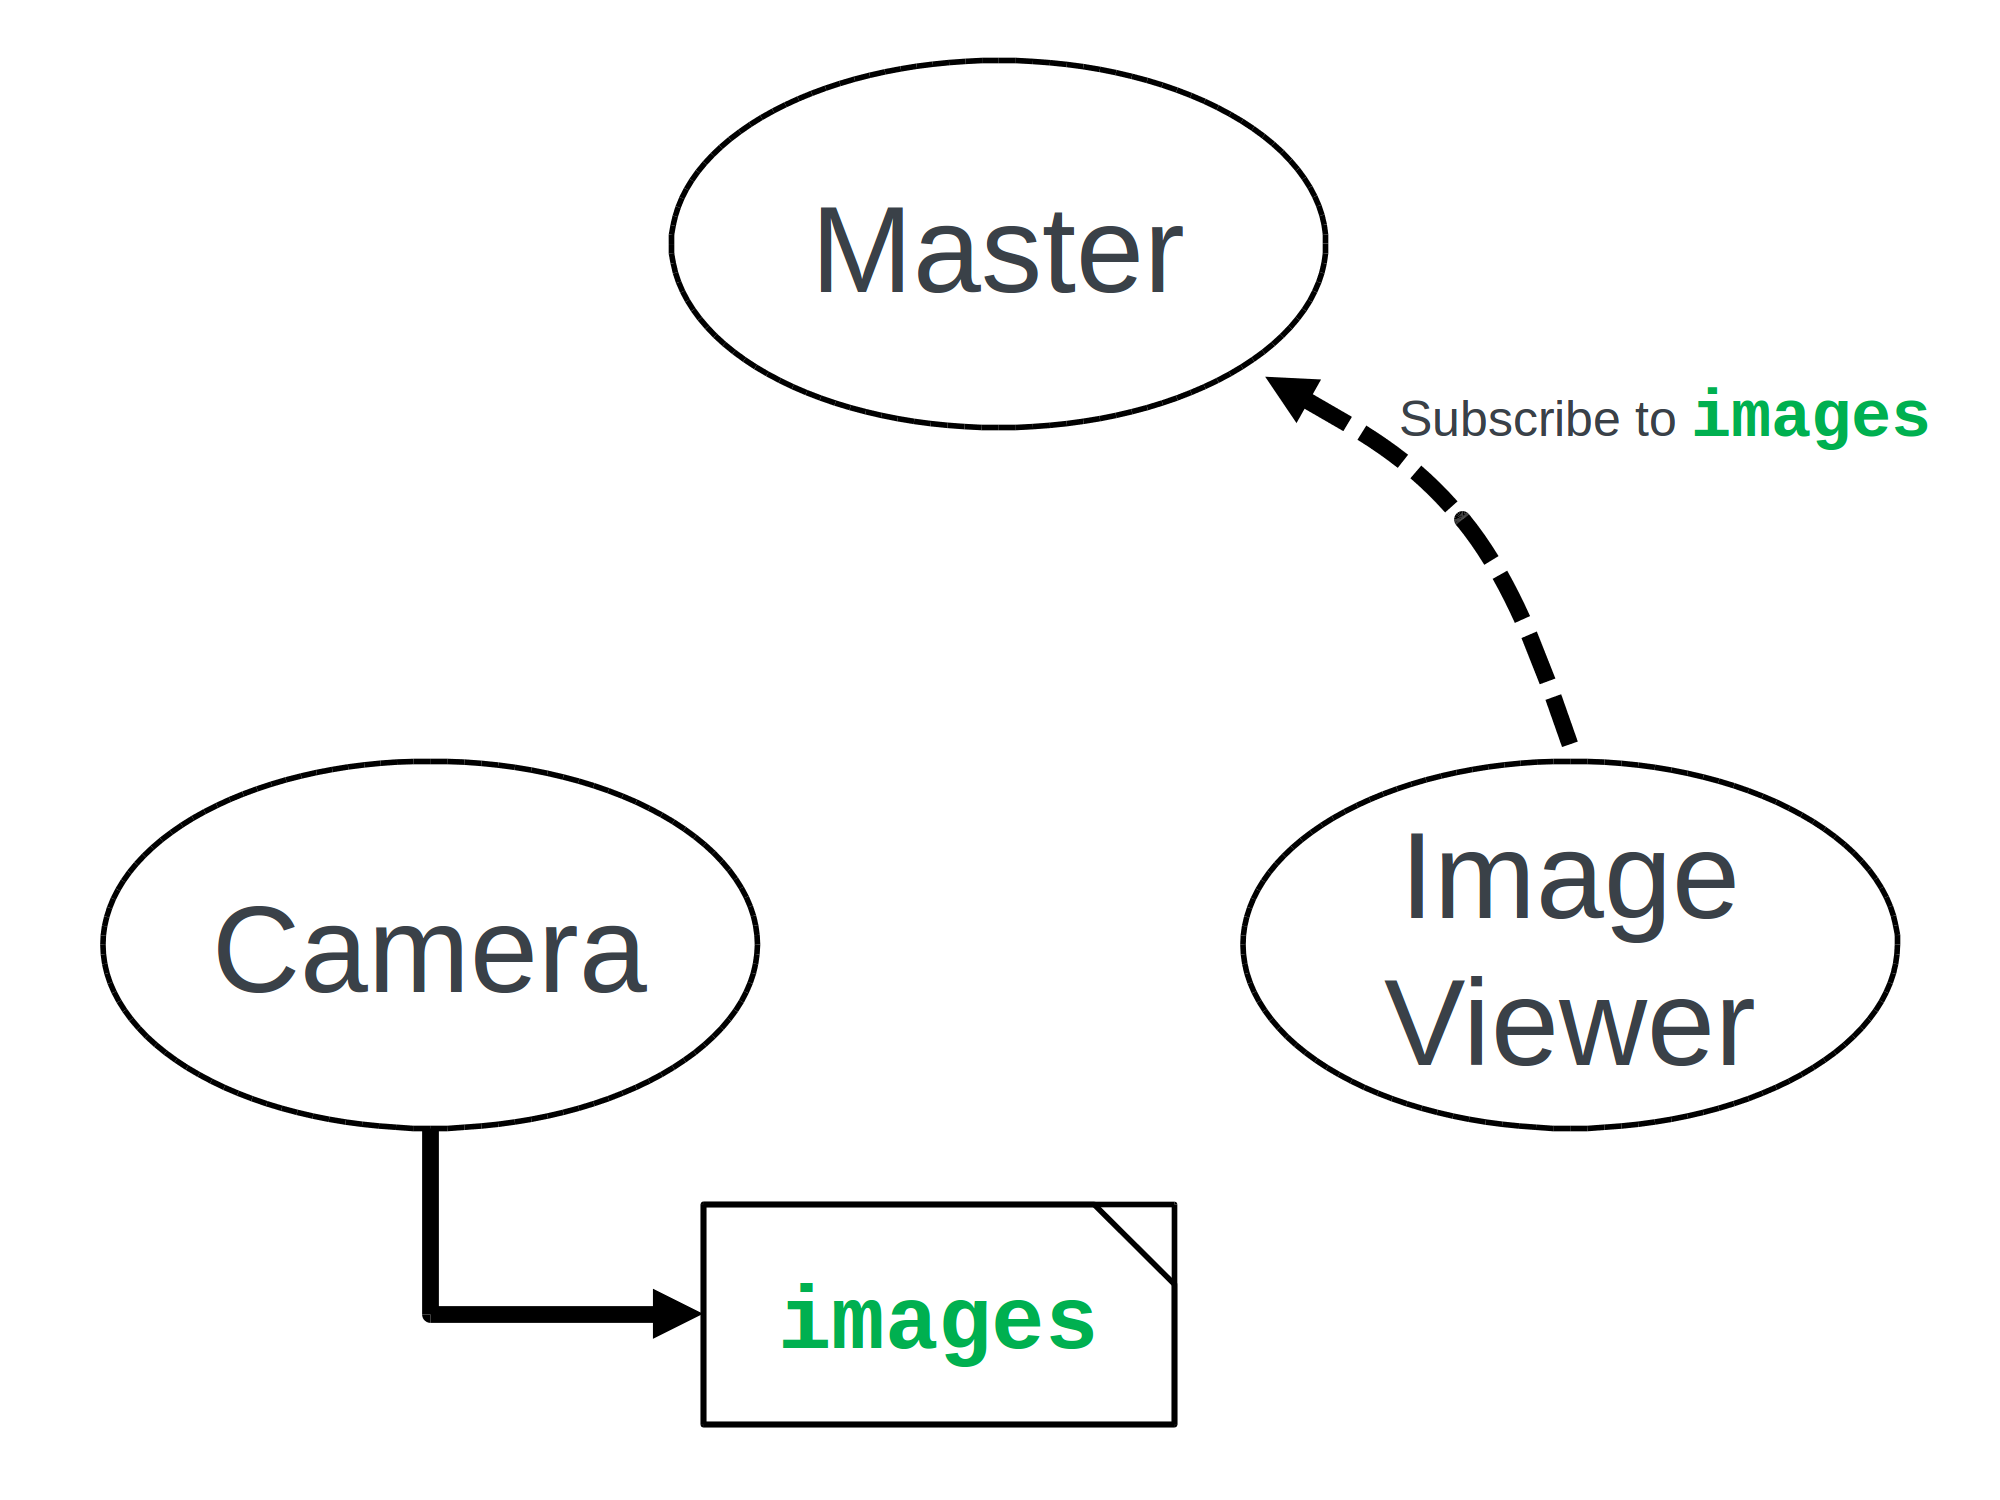
\includegraphics[width =1.0\linewidth]{figures/master3.png}                                                              
        \end{frame} 
        \begin{frame}[plain]{}
            \centering
            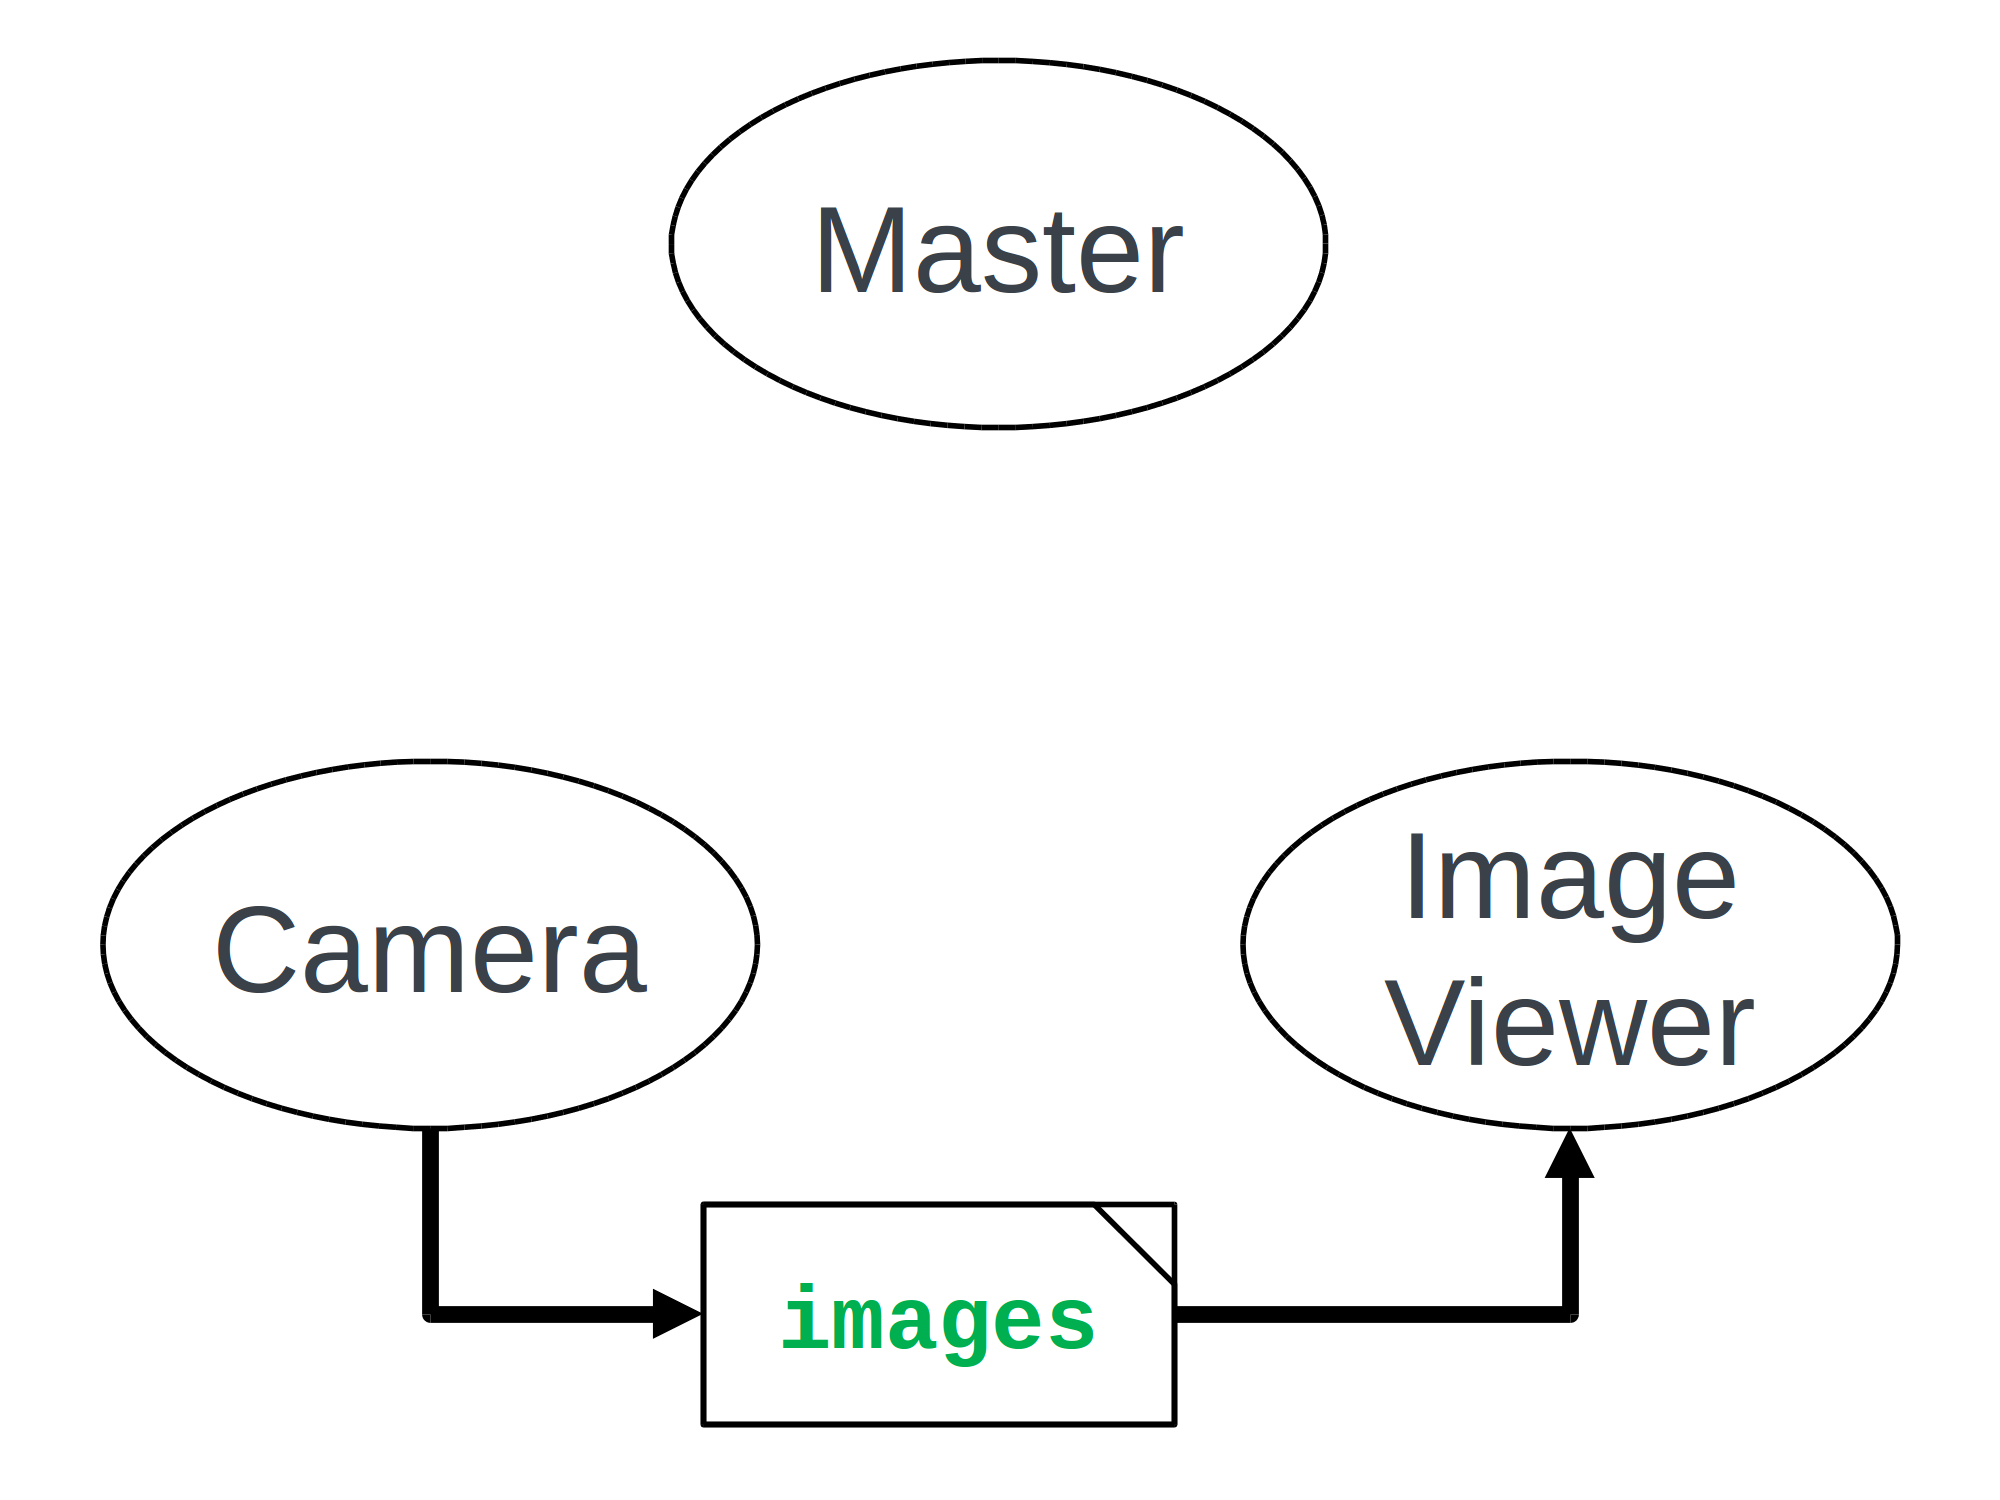
\includegraphics[width =1.0\linewidth]{figures/master4.png}                                                              
        \end{frame}
        
        

        
\section{ROS nodes in Python}

\subsection{A simple ROS node in Python}

\begin{frame}[fragile]{A simple ROS node}
    \framesubtitle{}
    \lstset{language=python,
        basicstyle=\ttfamily,
        keywordstyle=\color{blue}\ttfamily,
        stringstyle=\color{red}\ttfamily,
        commentstyle=\color{green}\ttfamily,
        morecomment=[l][\color{magenta}]{\#},
        showstringspaces=false
    }
    \begin{lstlisting}
#!/usr/bin/env python


import rospy
from time import sleep

rospy.init_node("print_text")


while True:
    print "Hello world!"
    sleep(1)
    \end{lstlisting}
\end{frame}


\begin{frame}[fragile]{A simple ROS node}
    \framesubtitle{ROS Nodes}
    \lstset{language=python,
        basicstyle=\ttfamily,
        keywordstyle=\color{blue}\ttfamily,
        stringstyle=\color{red}\ttfamily,
        commentstyle=\color{green}\ttfamily,
        morecomment=[l][\color{magenta}]{\#},
        showstringspaces=false
    }
\begin{lstlisting}
#!/usr/bin/env python

import rospy


rospy.init_node("print_text")  
rate = rospy.Rate(1)

while not rospy.is_shutdown():
    print "Hello world!"
    rate.sleep()
\end{lstlisting}
\end{frame}

\begin{frame}{Three ways to run a node}
    \framesubtitle{ROS Nodes}
    
    There are 3 ways to run a node:
    \begin{enumerate}
        \item Like you normally do. Example (in case of python node):
                \begin{terminal}
                \color{green} \ttfamily{python <file name>}
                \end{terminal}
        \item using rosrun command:
        \begin{terminal}
        \color{green} \ttfamily{rosrun <package name> <node name>}
        \end{terminal}
        
        \item Using launch files. \tiny{(we'll see it later)}

    \end{enumerate}
\end{frame}


\subsection{Writing a publisher node in Python}

\begin{frame}[fragile]{A simple ROS node}
    \framesubtitle{}
    \lstset{language=python,
        basicstyle=\ttfamily,
        keywordstyle=\color{blue}\ttfamily,
        stringstyle=\color{red}\ttfamily,
        commentstyle=\color{green}\ttfamily,
        morecomment=[l][\color{magenta}]{\#},
        showstringspaces=false
    }
\begin{lstlisting}

\end{lstlisting}
\end{frame}


\subsection{creating a package}
\begin{frame}{ROS Nodes}
    
\end{frame}










\end{document}
